\documentclass[20pt,margin=1in,innermargin=-4.5in,blockverticalspace=-0.25in]{tikzposter}
\geometry{paperwidth=48in,paperheight=36in}
\usepackage[utf8]{inputenc}
\usepackage{amsmath}
\usepackage{amsfonts}
\usepackage{amsthm}
\usepackage{amssymb}
\usepackage{mathrsfs}
\usepackage{graphicx}
\usepackage{adjustbox}
\usepackage{enumitem}
\usepackage[backend=biber,style=numeric]{biblatex}
\usepackage{mwe} % for placeholder images

% set theme parameters
\tikzposterlatexaffectionproofoff

\usecolorstyle{EmoryStyle}

%----------------------------------------------------------------------------------------
%	TITLE SECTION 
%----------------------------------------------------------------------------------------

\title{\textbf{Exponential Function \( f(x) = ab^x \)}} % Poster title

\author{\textbf{Manushree Mallaraju : 40082236}} % Author(s)

\institute{\textbf{Department of Software Engineering, Concordia University}} % Institution(s)

%----------------------------------------------------------------------------------------
% begin document
\begin{document}
\maketitle
\centering
\begin{columns}
    \column{0.32}
    \block{Introduction}{
         The funtion \( ab^x \)is one of the power rules of math, which involves an exponent. This exponent is represented with a variable rather than a constant, and its base is represented with constant value rather than a variable.\\
         \\$\bullet$~ Let \( f(x) = ab^x \) be an exponential function where “b” is its change factor (or a constant), the exponent “x” is the independent variable (or input of the function), the coefficient “a” is called the initial value of the function (or the y-intercept), and “f(x)” represent the dependent variable (or output of the function)\\
         \\$\bullet$~ This Poster Presentation describes the algorithms used to implement the function \( ab^x \), technical reasons for the selecting particular algorithm, lessons learnt during the project and the critical decisions made during the examining of the other team member's function.\\
         \\$\bullet$~ The domain is a set of all real numbers,R. where :\( b > 0 \) ,\( x > 0 \). The co-domain is also a set of all real numbers, R.\\

       }  
    
    
\block{Critical Decisions}{
   There were many situations which led to critical thinking:
   {\normalsize \textbf{1. To select an algorithm to implement the function. }}\\
   {\normalsize \textbf {Why this is critical $?$}}As there were several algorithms to implement the function, and algorithm has its own advantages and disadvantages. Where I analyzed the prons and cons of each algorithms and finally selected, Iterative Algorithm.
   
    \\$\bullet$~ Using Iterative algorithm is it easy to understand the flow of the program, where each step of the iteration is very clear.Whereas with Recursive, since the function calls itself, it is diffult to understand the flow of the program\\
    
    {\normalsize \textbf{2. Implementation :}}\\
    \\$\bullet$~ I found it difficult to implement the function, without using inbuilt math functions in Java. \\
     \\$\bullet$- Whenever the variable 'x' is a real number, it gives a decimal long value, where I need to calculate the power for the whole decimal number and result in run-time error. 
    \\$\bullet$~ To calculate the power of real number 'x', I had to understand the flow of Newton'n method of calculating Nth Root.
   \\$\bullet$~ Using Newton's method of Nth root calculation, it was easy to find the power of decimal long integer, where the digits were not rounded to its nearest value.
    
    {\normalsize \textbf{Code and Test Cases Review:}}\\
     \\$\bullet$~  As I had to completely understand the program flow of other function, where it took a long time. But it is very important to understand the flow of program to provide feedback to a team member.
     
     \\$\bullet$~ There are many tools to check the Code Review. I had to weigh the prons and cons of each Code Review tool to select a particular one.
\\
    }
    
    \column{0.36}
    \block{Graph of Exponential Function}{
         \begin{tikzfigure}[Figure: Graph of $ f(x) = ab^x $]
            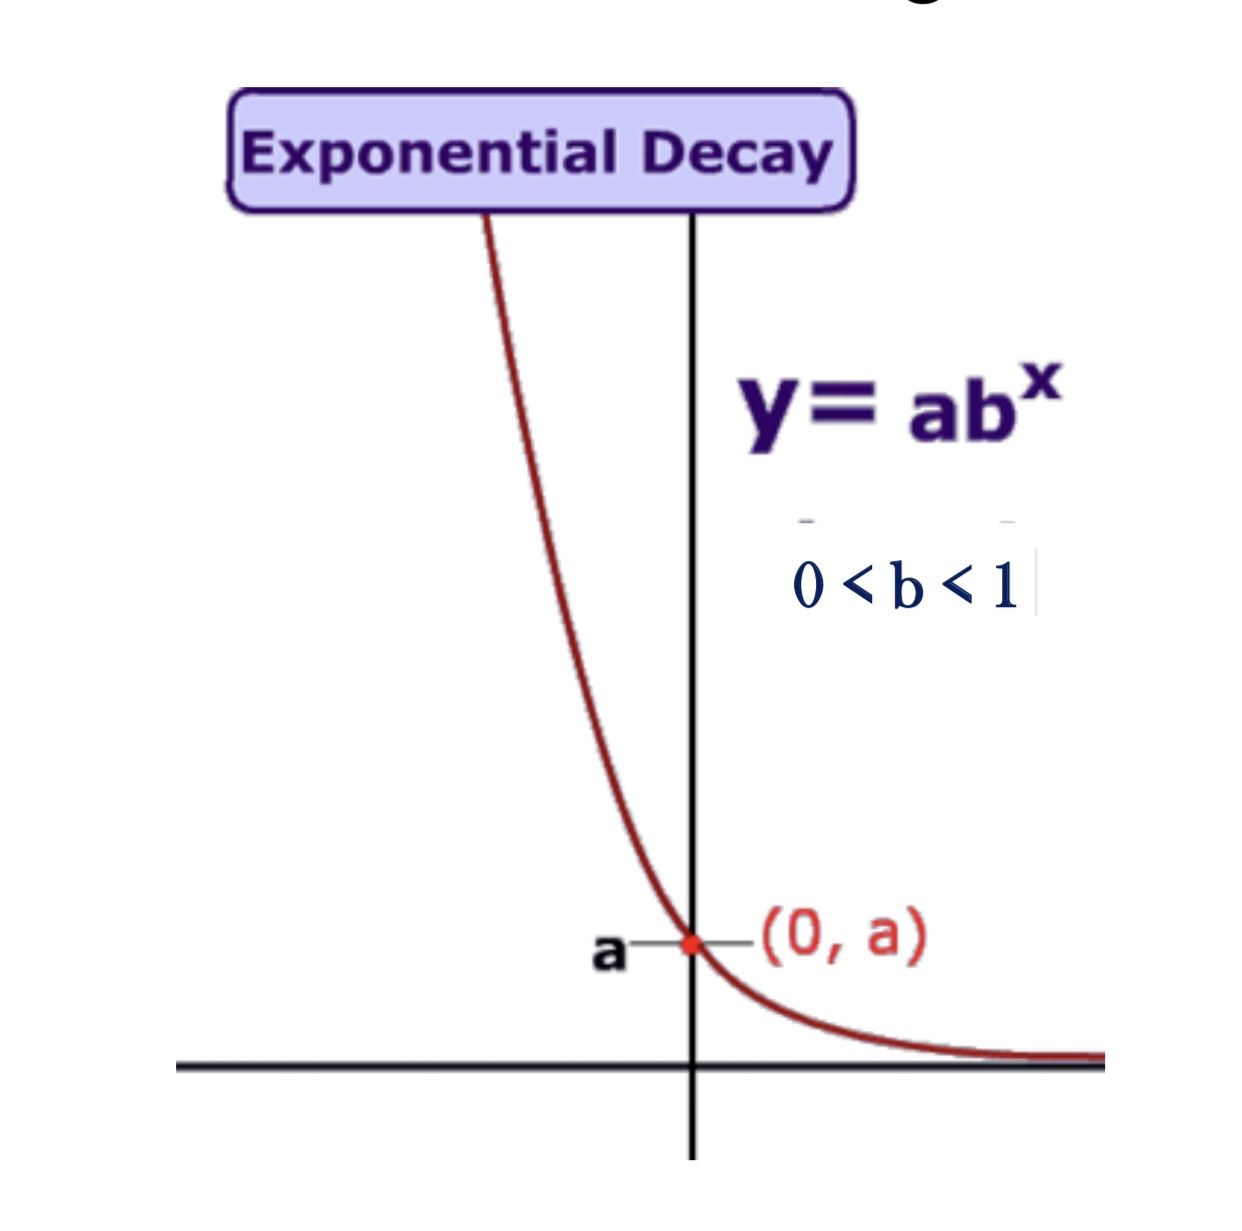
\includegraphics[width=0.5\linewidth]{PosterPresentation/IMG_1640.jpg}\\
        \end{tikzfigure}
        \\
    }

    \block{Challenges Faced }{
    There are number of challenges faced during the Project:
     \\$\bullet$~ As I am new to 'Latex', it was difficult for me to execute each and every Project Deliverable in Latex file. I learnt Latex from Scratch.\\
     \\$\bullet$~ I had basic knowledge of Java, but implementing Exponential functions without using inbuilt math functions was a bit challenging.\\
     \\$\bullet$~ In my function, Eventhough 'a' and 'b' are constants, calculating power of a real number 'x' was more challenging. As rounding of decimal numbers may not be accurate. Newton'n method of Nth Root, helped me to understand the flow of nth root function.
     }

    \block{Code Review }{
      \\$\bullet$~   I did the code review of Hina's F7 source code. The review were based on the four aspects: General, Requirements Coverage, Security and Documentation with reference from Google Coding Standards. \\
      \\$\bullet$~ During Source Code compilation, I found there are outputs which are printed which are not necessary. \\
      \\$\bullet$~ It was confusing for me to identify, 'which value is the actual result?'
      In few cases the output is not immediately displayed but it is displayed after few intermediate values are printed.
      \begin{tikzfigure}[]\\
            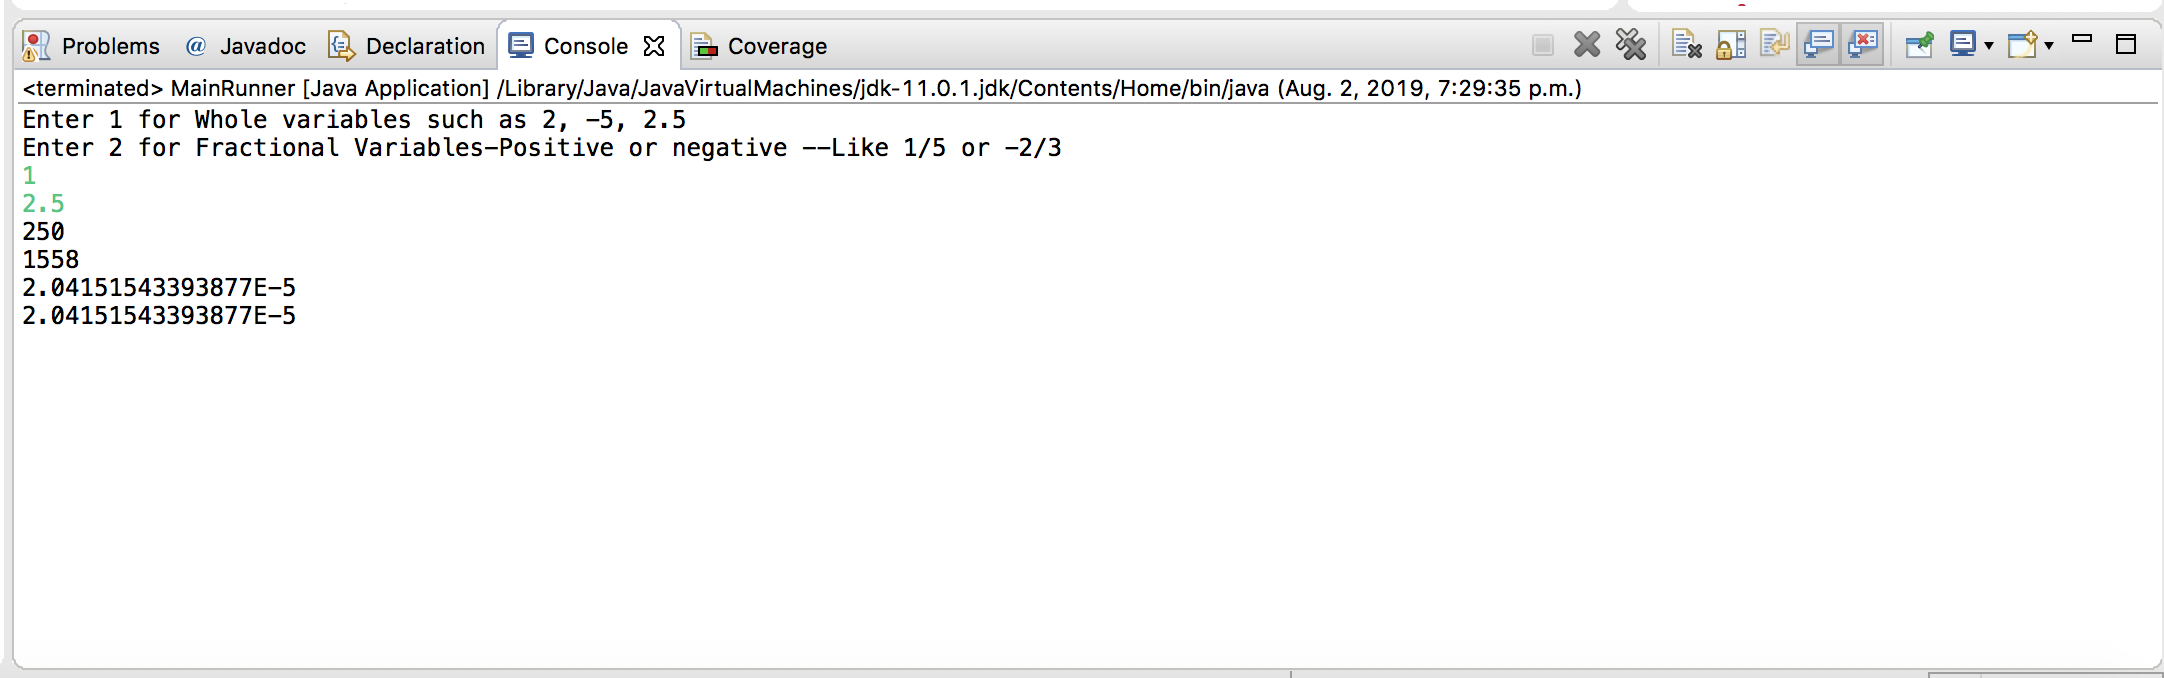
\includegraphics[width=1.0\linewidth]{PosterPresentation/SS.png}
        \end{tikzfigure}
        
    }
    
    \column{0.32}
    \block{Test Case Review}{
     I did the Test Case review of Jafar's function, F8 test.java. Test Cases are reviewed with the criteria how they achieve different coverages and analysis. \\
     
     Inputs used for review: Requirements Document and Java code, Java Test cases from Jafar's repository.
     
      \\$\bullet$~ Requirements of the Project was not at all met, it was difficult to Analyze the  flow of source code.\\
      
      \\
      \quad Requirement Coverage is required as part of Software Engineering Process to make ensure all the requirements are tested and validated in compliance with the given standards so as to achieve the desired behavior from the Program.\\
      \\
     }
   
    \block{Lessons Learned}{
        \\$\bullet$~ From the Test Case review and Code review, it is understood that we need to predefine a set of standards before starting to implement the design and test of the requirements. \\
        
       \\$\bullet$~The standards will help to maintain a particular format of coding and testing over the team. \\
        
       \\$\bullet$~ Code review helped identifying exceptions and dead code which might crash the implementation during run time. \\
       \\$\bullet$~ During the test case review, different possibilities of design going through can be identified and be tested to avoid exceptions during the run time.
      \\
      \\
    }
    
    \block{Overall Experience}{
        \\$\bullet$~ As I do not have any IT industry experience, I understood the process of 'How a Project will be executed in the Industry?'.\\
        
       \\$\bullet$~ Eventhough the Project is a small scale, we met each and every stage of Project Development Process. \\
        
       \\$\bullet$~ Learnt more about implementation, gained more knowledge with Newton's Method of Nth Root and also various Implementation methods of a Project. \\
       \\$\bullet$~ I went deep in understanding the Programming Language Java and using different types of Code Review tools, such as CheckStyle.
      \\
    }
 
    
\end{columns}
\end{document}
